\documentclass[hidelinks,12pt,a4paper]{report}
\usepackage[utf8]{inputenc}
\usepackage[english]{babel}
\usepackage{amsmath}
\usepackage{amsfonts}
\usepackage{amssymb}
\usepackage{graphicx}
\usepackage{gensymb}
\usepackage{hyperref}
\usepackage{array}
\usepackage{siunitx}
\usepackage[version=4]{mhchem}
\usepackage[style=authoryear, dashed=false, backend=biber, maxbibnames=99, giveninits=true,
citetracker=true, maxcitenames=2, natbib=true, terseinits=true, uniquename=false]{biblatex}
\usepackage{odsfile,booktabs}
\usepackage{lscape}
\usepackage{pdflscape}
\usepackage{longtable}
\usepackage{chemfig}
\usepackage{heuristica}
\usepackage[heuristica,vvarbb,bigdelims]{newtxmath}
\usepackage[T1]{fontenc}
\renewcommand*\oldstylenums[1]{\textosf{#1}}
%\usepackage{fontspec}
%\setmainfont{QTPalatine}
\usepackage[hang, bf, small]{caption}
\usepackage{tabularx}
\usepackage{footnote}
%\usepackage{tikz}
\usepackage[edges]{forest}
\usetikzlibrary{positioning,arrows}
\usepackage{graphicx}
\usepackage{geometry}



\DeclareSIUnit\au{AU}
\DeclareSIUnit\mgpl{\milli\gram\per\liter}
\DeclareSIUnit\mgg{\milli\gram\per\gram}
\DeclareSIUnit\cell{cell}

\title{Microbial Pb(II) removal: modelling the role of passive mechanisms}
\author{Brandon van Veenhuyzen}
\addbibresource{MEng.bib}


\begin{document}
	
	\maketitle
	\tableofcontents
	
	\chapter{Theory}

\section{Background}

\subsection{Lead and the environment}

Five million tons of lead (Pb) ore are mined annually to be refined for use in a variety of industrial applications \parencite{ILA2019}. The most common application of Pb is in the manufacturing of Pb acid batteries for energy storage. These batteries are mostly utilized in automotive applications as well as emergency power supplies for various critical services such as hospitals, communication networks, public buildings, and emergency services. Additionally, Pb batteries arguably form the backbone of renewable energy industries such as solar photo-voltaic implementations, wind turbines, and electric or hybrid vehicles. The extremely high density of Pb provides unrivalled radiation protection which is essential for medical, dental, research, and nuclear installations. Further, Pb is used as a stabilizer to increase the durability of PVC products and has been applied to thousands of kilometres of underwater power and communication cabling \parencite{ILA2019}.

Two problems, however, arise from lead industries. Firstly, the present rate of lead extraction considered with the most recent estimate of current lead ore reserves (\SI{88}{\mega\tonne}) means that raw lead could potentially be depleted by 2035 \parencite{Statista2019}. Secondly, these industries introduce lead pollutants into the environment. This includes drainage and tailings from mining, waste water streams and spillage from processing, and landfill leachate from the disposal of Pb-containing products \parencite{UNEP2010, VanHille}. The most concerning form of lead pollution is in ionic or aqueous form: Pb(II). In this oxidation state it is soluble in water and more likely to form organic complexes or attach to colloidal particles, making it exceptionally mobile and available for interference in biological processes \parencite{Naik2013}. A compilation of sampled effluent Pb(II) concentrations are given in Table~\ref{tab:industrial-lead}. 

\begin{table}[htbp!]
	\setlength{\extrarowheight}{0.1cm}
	\caption{Concentration of aqueous lead in various industrial waste waters. Source: \textcite{Verma2016}.}
	\label{tab:industrial-lead}
	\centering
	\begin{small}
\begin{tabular}{>{\raggedright\arraybackslash}m{6cm}>{\centering\arraybackslash}m{4cm}}
	\toprule 
	Industry & Effluent concentration (\si{\milli\gram\per\liter} \ce{Pb^2+}) \\ 
	\midrule 
	Chemical manufacturing plant & 326 \\
	Oil & 125 - 250   \\ 
	Battery manufacturing & 5 - 15   \\ 
	Electroplating & 116   \\ 
	Industrial plant & 19.1 \\
	\bottomrule
\end{tabular} 
\end{small}
\end{table}

Lead is highly toxic and has been found to accumulate through different trophic levels of ecosystems \parencite{Naik2013}. Lead could therefore be present in sub-lethal quantities in water but concentrate to lethal doses within the food chain \parencite{VanHille}. Lead serves no biological purpose, but rather harms organisms by disrupting the electron transport chain \parencite{Okoro2011}, damaging membranes \parencite{Patra2011} and denaturing proteins \parencite{Gadd1977}, impairing enzymes \parencite{Yang2006}, and substituting cationic nutrients \parencite{Okoro2011}. Exposure to toxic heavy metals has also been found to stunt growth in organisms as cellular energy is redirected towards mechanisms of repair and resistance \parencite{Knops2001}. In plants, lead exposure results in necrosis, the inhibition of growth, and a reduction in biomass \parencite{Shakoor2013}. For animals, this harm is seen in the form of damage done to the central nervous system, kidneys, reproductive and immune system \parencite{UNEP2010}.

Cases of lead poisoning have been reported in local communities close to lead-acid battery recycling plants, lead transportation routes, and lead ore mines \parencite{Shakoor2013}. In humans, exposure to high concentrations of lead has been shown to cause neuronal encephalopathy and gastrointestinal colic, which includes symptoms such as constipation, abdominal pain, and intestinal paralysis \parencite{Mudipalli2007}.  

Lead, lead dioxide, and lead sulfate are classified as very or extremely hazardous wastes in South Africa. These compounds are considered to pose acceptable risks in the environment only at concentrations below \SI{0.1}{\milli\gram\per\liter} and can only be disposed of at a monthly amount of less than \SI{151}{\gram\per\hectare} in an immobilised or encapsulated form \parencite{DWAF1998}. Guidelines for the upper limit of lead in water for various uses are given in Table~\ref{tab:dwaf}.
\begin{table}[htbp!]
	\setlength{\extrarowheight}{0.1cm}
	\caption{Water quality targets for lead in various uses of water. Adapted from \textcite{DWAF1998}.}
	\label{tab:dwaf}
	\centering
	\begin{small}
	\begin{tabular}{l>{\centering\arraybackslash}m{4cm}}
		\toprule
		Category of water use & Upper limit (\si{\milli\gram\per\liter}~\ce{Pb^2+}) \\
		\midrule
		Domestic & 0.01 \\
		Irrigation & 0.2 \\
		Livestock watering &  0.1 \\
		Aquatic ecosystems & 0.06 \\
		\bottomrule
	\end{tabular}
	\end{small}
\end{table}



\subsection{Current heavy metal removal technology}

Various processes are available to remove Pb(II) from industrial effluent. A summary of the most widely employed techniques is presented in Table~\ref{tab:conventional}. Although the established use of these methods make them favourable, recurring disadvantages of these processes include high operating and maintenance costs as well as the need to further treat the concentrate of heavy metal produced.


\begin{small}
\setlength{\extrarowheight}{0.2cm}
\begin{longtable}{>{\raggedright\arraybackslash}p{2.5cm}>{\raggedright\arraybackslash}p{3cm}>{\raggedright\arraybackslash}p{3cm}>{\raggedright\arraybackslash}p{3cm}}
	\caption{Conventional techniques employed for removing heavy metal from water. Compiled from \textcite{Fu2011a}, \textcite{VanHille}, and \textcite{Edzwald2011}.}
	\label{tab:conventional}\\
	\toprule
	Treatment strategy & Description & Advantages & Disadvantages \\ 
	\midrule
	\endhead
	\bottomrule
	\endfoot
	Chemical precipitation & Compounds are added to water to react heavy metals into a less soluble form. & Fast kinetics, simple operation. & Sludge generation and poor efficiency with effluents of low metal concentration. \\ 
	Ion exchange & Heavy metals are swapped for benign counter-ions from an exchange resin. & Rapid operation, high selectivity and treatment capacity. & Sensitive to sulfates and dissolved solids, large volumes of regenerant to be disposed of. \\ 
	Pressure driven membrane filtration & Treatments such as reverse osmosis that force water through a membrane which rejects heavy metals. & High efficiency and selectivity. & High operating and maintenance costs. Heavy metal concentrate requires safe disposal. \\ 
	Adsorption & Heavy metals in the aqueous phase bind to the surface of a solid. & Low capital cost, solids can be regenerated. & Low selectivity. Desorption process required to recover heavy metals. \\ 
	Electrochemical treatment & An applied current causes the deposition of heavy metals onto an electrode. & Recovery of metal in metallic form. & High operating costs. \\ 
	Electrodialysis & Membrane process driven by electric potential to remove heavy metal. & High recovery of water. & High operating costs. Heavy metal concentrate requires disposal. \\ 
\end{longtable}
\end{small}

\subsection{Bioremediation and biorecovery of aqueous lead by local lead-resistant organisms}

A promising alternative to conventional technology for the removal of aqueous \ce{Pb} is bioremediation, where organisms are used to remove or detoxify the heavy metal \parencite{Philp2005}. Bioremediation is attractive due to the variety of biomaterials applicable (such as algae, fungi, plants, and bacteria) and its potential for low cost and high efficiency operation at low \ce{Pb} concentrations \parencite{Kang2015}. \ce{Pb} removal with organisms has mostly been limited to sorption with biomass \parencite{Chatterjee2012}, the use of plants for phytoextraction \parencite{Shakoor2013}, and fungi for mycelial biosorption \parencite{Chakraborty2013}. Some microorganisms have been discovered that reduce the bioavailability and toxicity of \ce{Pb} by precipitating it out as an insoluble complex. \textit{Staphylococcus aureus}, for example, has been found to take up \ce{Pb(II)} and precipitate it out as \ce{Pb_{3n}(PO4)_{2n}}  crystals \parencite{Levinson1996,Naik2013}. Additionally, several species of Pb-resistant marine bacteria tend to form insoluble \ce{PbS} \parencite{De2008} when exposed to \ce{Pb(II)}. 

Several subterranean anaerobic bacteria have been reported to respire using a range of terminal electron acceptors, including heavy metal pollutants \parencite{Haas2001}. Respiration involving the reduction of soluble oxidised-metals can lessen the mobility of the metal.

A consortium of bacteria has been isolated from lead-contaminated soil at a battery recycling plant in Gauteng, South Africa, that has been shown to remove \ce{Pb(II)} from solution \parencite{Brink2017}. This lead-resistant consortium has been the subject of many investigations in the pursuit of better understanding the removal mechanisms and possible implementations in the bioremediation and biorecovery of lead in industrial effluent. This includes studies on the influence of lead concentrations \parencite{Brink2017,Peens2018d}, substrate concentration \parencite{Brink2017,Brink2018}, precipitate identification \parencite{Brink2019a,Peens2018}, and the influence of Zn(II) and Cu(II) concentrations \parencite{Horstmann2020}. Key findings in the investigations are outlined in this section.  

\subsubsection{Consortium characterisation}

Streak and spread plates were prepared for the lead resistant culture at 80 and \SI{500}{\milli\gram\per\liter} \ce{Pb(II)}. The streak plate analyses was used to confirm the presence and abundance of species in the consortium using sequencing and analysis from the Basic Local Alignment Search Tool (BLAST). In the spread plates, colonies exhibiting precipitate formation were isolated before being sequenced and analysed using 16s rRNA genetic fingerprinting in order to identify dominant bacteria. 

The streak plates showed that at \SI{80}{\milli\gram\per\liter}  \textit{Enterococcus} sp. and \textit{Clostridium botulinum} were present in the largest quantity, but at 500 ppm Pb(II), \textit{Ralstonia solanacearum} and \textit{Klebsiella pneumoniae} were the most abundant. Furthermore, \textit{Klebsiella pneumoniae} was identified as the dominant bacteria in spread plate isolates from both 80 and \SI{500}{\milli\gram\per\liter} \parencite{Peens2018}.

\subsubsection{Lead precipitation}

Analysis revealed that \ce{PbS} made up approximately \SI{80}{\percent} of the precipitate formed when the culture was exposed to \SI{80}{\milli\gram\per\liter} \ce{Pb(II)} and \SI{40}{\percent} at \SI{500}{\milli\gram\per\liter} \parencite{Peens2018}. A study into the minimum inhibitory \ce{Pb(II)} concentration of the culture identified the precipitate ratio of \ce{PbS}:\ce{Pb} as 0.82:0.18 in batch processes, confirming the production of elemental lead by the consortium.


  

\subsubsection{Modelling microbial kinetics}

\textcite{Horstman2019} studied the kinetic behaviour of the consortium over \SI{33}{\hour} and \SI{15}{\day} periods in batch reactors with varied substrate and \ce{Pb(II)} initial concentrations. Kinetic models for \ce{Pb(II)} removal and growth kinetics were developed.

The lead-removal model was formed on several assumptions based on experimental data, namely that growth and substrate concentration do not affect the removal rate and that removal occurs in separate fast and slow mechanisms. The model is presented in Equation~\ref{eq:carla-kin}: 
\begin{equation}
	-\frac{dC}{dt} = \left( \frac{k_m C }{C + K_c}\right)_\textrm{fast} + \left( \frac{k_m C }{C + K_c}\right)_\textrm{slow} \label{eq:carla-kin}
\end{equation}
Where $ C $ is the concentration of \ce{Pb(II)} in \si{\milli\gram\per\liter}, $ t $ is time in \si{\day}, $ k_m $ is the maximum reduction rate in \si{\milli\gram\per\liter\per\day}, and $ K_c $ is the half-velocity constant in \si{\milli\gram\per\liter}. The integrated form of Equation~\ref{eq:carla-kin} is given in Equation~\ref{eq:carla-kin-int}:
\begin{equation}
	C(t) = C_0 \left[ \phi e^{\alpha_\textrm{fast}} +  \left(1 - \phi \right) e^{\alpha_\textrm{slow}} \right] \label{eq:carla-kin-int}
\end{equation}
Here, $ C_0 $ is the initial concentration of \ce{Pb(II)} in \si{\milli\gram\per\liter}, $ \phi $ is the fraction of lead removal involved in the fast phase, and $ \alpha = \frac{k_m}{K_c} $ for either the slow or fast phase. Parameters estimated for the kinetics of \ce{Pb(II)} removal are given in Table~\ref{tab:carla-pb}.
\begin{table}[htbp!]
	\caption{Constants fit by \textcite{Horstman2019} for Equation~\ref{eq:carla-kin-int}.}
	\label{tab:carla-pb}
	\centering
	\begin{small}
	\begin{tabular}{ll}
		\toprule
		$ \phi $ & 0.596 \\
		$ \alpha_\textrm{fast} $ & 17.39  \\
		$ \alpha_\textrm{slow} $ & 0.0436  \\
		\bottomrule
	\end{tabular}
	\end{small}
\end{table}

A model for consortium growth was proposed based on metabolic activity readings. Metabolic activity  was measured with 3-(4,5-dimethylthiazol-2-yl)-2,5-diphenyl tetrazolium bromide, or MTT. MTT is a yellow dye that is reduced to formazan crystals by the dehydrogenase system of viable Gram-negative bacterial cells. MTT is added to a reactor sample and incubated for an hour, after which formazan crystals are dissolved by dimethyl sulfoxide. A spectrophotometer with light at \SI{550}{\nano\meter} is thereafter used to quantify the amount of light absorbed by formazan and  infer metabolic activity.

Growth modelling was split into three consecutive phases, focusing on changes in biomass with dominant influences from nitrates, substrate, and the death of cells. These three factors are accounted for in Equation~\ref{eq:dxdt}.
\begin{align}
\frac{dX}{dt} = \left(\frac{dX}{dt}\right)_\textrm{\ce{NO3}} + \left(\frac{dX}{dt}\right)_\textrm{subst} + \left(\frac{dX}{dt}\right)_\textrm{death} \label{eq:dxdt}
\end{align}
Where $ X $ is the biomass concentration in \si{\au} (absorbance units). The phase initially observed is nitrate dependent is modelled on Monod kinetics as:
\begin{align}
	\left(\frac{dX}{dt}\right)_\textrm{\ce{NO3}} = \left[\frac{\mu_\textrm{max}}{1 + \frac{C}{K_i}}\right] \left( \frac{N - N_\textrm{crit}}{k_S + N - N_\textrm{crit}} \right) X \label{eq:x-nit} 
\end{align}
Here, $ \mu_\textrm{max} $ is the maximum specific growth rate in \si{\per\day},  $ K_i $ is the \ce{Pb(II)} inhibition constant in \si{\milli\gram\per\liter}, $ N $ is the concentration of \ce{NO3-} in \si{\gram\per\liter}, $ N_\textrm{crit} $ is the critical concentration of \ce{NO3-} in \si{\gram\per\liter}, and $ k_S $ is the half velocity constant in \si{\milli\gram\per\liter}. Parameters estimated for the kinetics of nitrate dependant growth are given in Table~\ref{tab:x-nit}.

\begin{table}[htbp!]
	\caption{Constants fit by \textcite{Horstman2019} for Equation~\ref{eq:x-nit}.}
	\label{tab:x-nit}
	\centering
	\begin{small}
	\begin{tabular}{lc}
		\toprule
		$ \mu_\textrm{max} $ & \SI{28.2}{\per\day} \\
		$ k_s $ & \SI{0.01}{\milli\gram\per\liter}  \\
		$ K_i $ & \SI{498.8}{\milli\gram\per\liter}  \\
		$ N_\textrm{crit} $ & ?? \\
		\bottomrule
	\end{tabular}
\end{small}
\end{table}

The relationship between nitrates and growth is also described in this phase as:
\begin{equation}
	\frac{dX}{dt} = Y_{XN} \frac{dN}{dt}
\end{equation}
Where $ Y_{XN} $ is the yield of biomass from nitrates in \si[inter-unit-product=\ensuremath{{}\cdot{}}]{\au\liter\per\gram}. \textcite{Horstman2019} found that at $ C_0 = \SI{500}{\milli\gram\per\liter}$ then $ Y_{XN} = \SI[inter-unit-product=\ensuremath{{}\cdot{}}]{0.0487}{\au\liter\per\gram} $, whereas at $ C_0 = \SI{80}{\milli\gram\per\liter}$ then $ Y_{XN} = \SI[inter-unit-product=\ensuremath{{}\cdot{}}]{0.0110}{\au\liter\per\gram} $.

A logistic differential model is used to describe the second phase of growth enhanced by substrate: 
\begin{equation}
	\left(\frac{dX}{dt}\right)_\textrm{subst} = \mu_\textrm{max} X \left(\frac{K- X}{K}\right) \label{eq:carla-logistic}
\end{equation}
Where $ K $ is the biomass carrying capacity of the system in \si{\au}. Cultures grown with initial concentrations of \SI{80}{\milli\gram\per\liter} \ce{Pb(II)} and \SI{25}{\gram\per\liter} substrate showed no substrate enhanced growth, whereas the parameters for cultures grown at double that initial substrate concentration and \SI{500}{\milli\gram\per\liter} \ce{Pb(II)}  are given in Table~\ref{tab:carla-logistic}.

\begin{table}[htbp!]
	\caption{Constants fit by \textcite{Horstman2019} for Equation~\ref{eq:carla-logistic} at initial conditions of \SI{10}{\gram\per\liter} yeast extract, \SI{20}{\gram\per\liter} tryptone, \SI{1}{\gram\per\liter} \ce{NaCl}, and \SI{500}{\milli\gram\per\liter} \ce{Pb(II)} at the start of enhanced growth phase.}
	\label{tab:carla-logistic}
	\centering
	\begin{small}
	\begin{tabular}{lc}
		\toprule
		$ X_0 $ & \SI{8.27}{\au}  \\
		$ \mu_\textrm{max} $ & \SI{9.88}{\per\day} \\
		$ K $ & \SI{13.23}{\au}  \\
		\bottomrule
	\end{tabular}
\end{small}
\end{table}

The final phase in the model uses one-phase decay to describe the death of cells as:
\begin{equation}
	\left(\frac{dX}{dt}\right)_\textrm{death} = - K_d X \label{eq:carla-death}
\end{equation}
With $ K_d $ being a constant in \si{\per\day}. The parameters estimated for the death phase of two experimental runs are given in Table~\ref{tab:carla-death}.

\begin{table}[htbp!]
	\caption{Constants fit by \textcite{Horstman2019} for Equation~\ref{eq:carla-death} from the biomass concentration at the start of the death phase ($ X_{d0} $) until equilibrium $ X_f $.}
	\label{tab:carla-death}
	\centering
	\begin{small}
	\begin{tabular}{>{\centering\arraybackslash}m{0.15\columnwidth} >{\centering\arraybackslash}m{0.27\columnwidth} >{\centering\arraybackslash}m{0.14\columnwidth} >{\centering\arraybackslash}m{0.14\columnwidth} >{\centering\arraybackslash}m{0.14\columnwidth}}
		\toprule
		$ C_0 $ (\si{\milli\gram\per\liter}) & Initial substrate ( \si{\gram\per\liter}, excl. \ce{NaCl}) & $ X_{d0} $ (\si{\au})& $ X_f $ (\si{\au})& $ K_d $ (\si{\per\day})\\
		\midrule
		80 & 15 & 8.77 & 4.09 & 0.594 \\
		500 & 30 & 13.25 & 6.682 & 0.4136 \\
		\bottomrule
	\end{tabular}
\end{small}
\end{table}

\subsubsection{Continuous reactor}

\textcite{Chimhundi2020} used the consortium in a continuous upflow anerobic sludge blanket reactor (CUASBR). The reactor demonstrated half the contact time necessary for lead reduction when compared to batch processes but only achieved \SI{0.03}{\percent} lead recovery. New precipitates identified from the reactor include apatite and pyromorphite. 

Shock loading in the CUASBR also demonstrated the ability of the consortium to  survive at concentrations of \SI{2000}{\mgpl}.

\section{The role of biosorption}

The model presented in Equation~\ref{eq:carla-kin} for the removal of \ce{Pb(II)} does not distinguish between metabolically active processes of and the passive adsorption of lead onto cell walls. Literature, however, suggests that the fast phase in Equation~\ref{eq:carla-kin} could be attributed to a rapid initial phase of biosorption. This is backed up by findings such as Pb(II) adsorption onto yeast reaching equilibrium after 6 minutes \parencite{DuncanJ.R.2003}, 95 \% Pb(II) removal after 60 seconds by the algae \textit{Spirulina} sp. \parencite{VanHille}, and Cu(II) adsorption reaching equilibrium in 30 minutes \parencite{LawrenceR.W.BranionR.M.R.&Ebner}. This section discusses biosorption and its possible role in \ce{Pb(II)} removal by the battery recycling plant consortium.

\parencite{Qin2020} Existing research shows that heavy metal removal takes place in two steps. The first step is metaolically independent and takes place on the surface of the cell, can also be done by dead bacteria. Physi, IX, and Surfcomplex.. Second phase involves surface microprecipitation and internal accumulation which require celluar energy

\subsection{Introduction}

In waste water treatment, adsorption describes a mass transfer process whereby pollutants are transferred from out of the liquid phase onto a solid surface \parencite{Wang2020}. It is widely regarded as one of the most effective forms of advanced waste water treatment \parencite{KumarReddy2012}, and is generally seen as both simple to implement and cost effective \parencite{Fomina2014}. 

Biosorption is an umbrella term involving physico-chemical adsorption mechanisms to materials of biological origin \parencite{Robalds2016}. Authors usually use the term exclusively for metabolically independent processes \parencite{Fomina2014}, in contrast to the non-passive mechanisms involved with bioaccumulation. The key biosorption terminology encountered in literature and used in this dissertation is summarised in Figure~\ref{fig:terminology}. Sorption terms prefixed with \textit{bio-} are frequently used interchangeably with terms prefixed with \textit{ad-} within the confines of biosorption discussions.

\begin{figure}[tbph!]
	\centering
	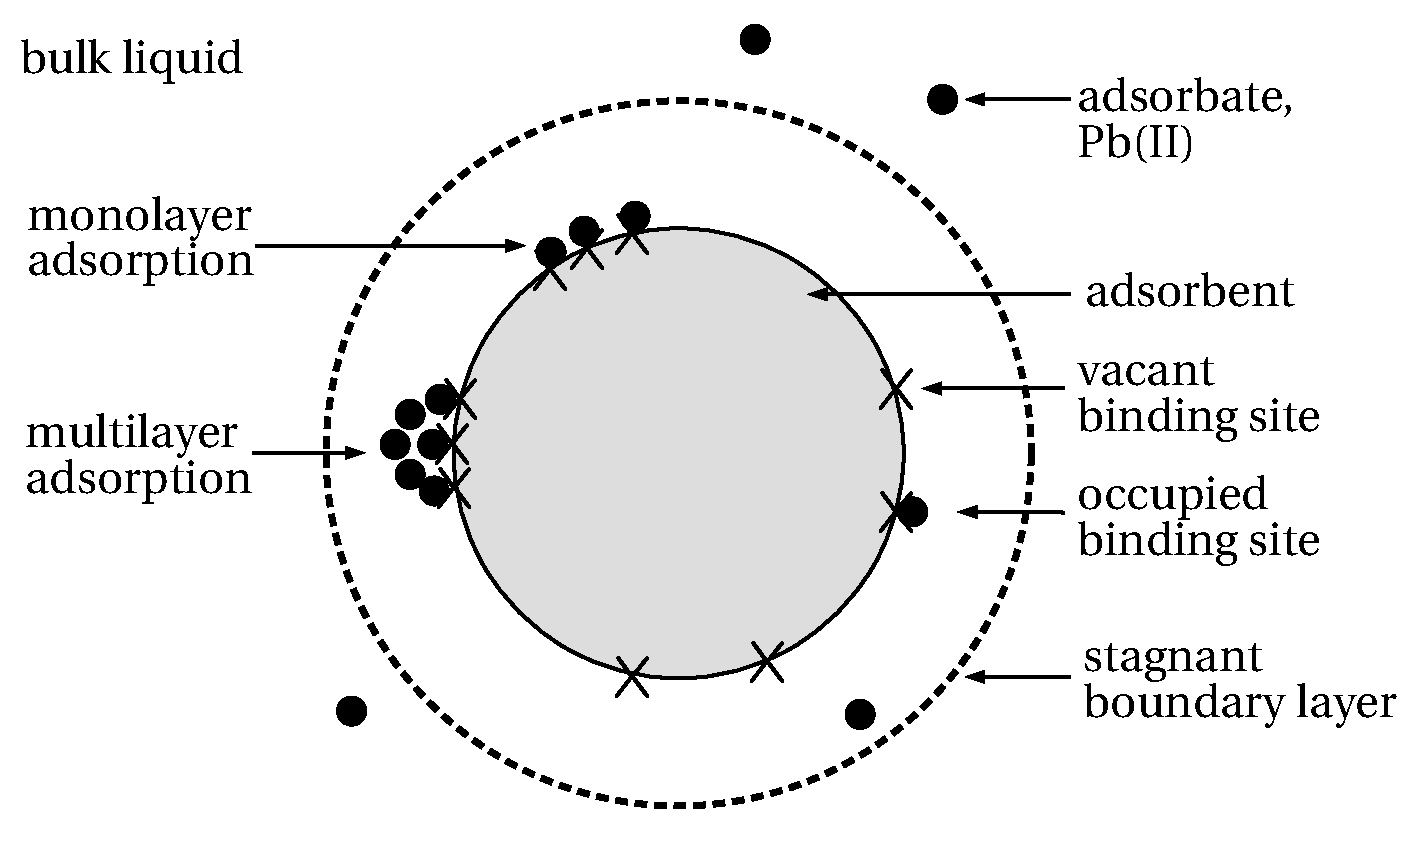
\includegraphics[width=0.8\linewidth]{Theory/Pics/terminology}
	\caption{Visualisation of basic adsorption terminology. Adapted from \textcite{Tran2017}}
	\label{fig:terminology}
\end{figure}

Adsorbents are primarily evaluated by how much adsorbate is retained by the material. This referred to as the uptake or adsorption capacity, and is calculated as \parencite{Volesky2007}:
\begin{align}
\label{eq:1}
q=\frac{\left(C_0-C\right)V}{W}
\end{align}
Where $ q $ is the adsorption capacity in \si{\mgpl}, $ V $ is the volume of adsorbate-bearing solution in \si{\liter}, and $ W $ is the dry mass of adsorbent in \si{\milli\gram}. The lead uptake calculated for a variety species of bacteria found in literature is given in Table~\ref{tab:qbact}.

\begin{table}[htbp!]
	\centering
	\caption{Biosorption capacity of \ce{Pb(II)} onto various species of bacteria.}
	\label{tab:qbact}
	\begin{small}
		
	
	\begin{minipage}{\textwidth}
	\begin{tabularx}{\textwidth}{>{\raggedright\arraybackslash}X>{\centering\arraybackslash\hsize = 0.5\hsize}XX}
		\toprule
		Species & \ce{Pb(II)} uptake (\si{\milli\gram\per\gram}) & Reference \\
		\midrule
		
		\textit{Acinetobacter junii} L. Pb1 & 165 & \textcite{Kushwaha2017} \\
		\textit{Arthrobacter sp.} & 130 & \textcite{Veglio1997} \\
		\textit{Bacillus} sp. (ATS-1) & 92.3 & \textcite{Tunali2006} \\
		\textit{Bacillus} sp. PZ-1 & 9.30 & \textcite{Ren2015} \\
		\textit{Bacillus firmus}\textsuperscript{a} & 1100 & \textcite{Salehizadeh2003} \\
		\textit{Corynebacterium glutamicum} & 568 & \textcite{Choi2004} \\
		\textit{Curtobacterium} sp. FM01 & 187 & \textcite{Masoumi2016} \\
		\textit{Enterobacter} sp. J1 & 50.0 & \textcite{Lu2006} \\
		\textit{Enterobacter cloacae} & 2.30 & \textcite{Ayangbenro2017}\\
		\textit{Micrococcus luteus} DE2008\textsuperscript{b} & 1965 & \textcite{Puyen2012} \\
		\textit{Pseudomonas} sp. LKS06 & 77.8 & \textcite{Huang2013}\\
		\textit{Pseudomonas aeruginosa} PU21 & 0.735 & \textcite{Lin2006a} \\
		\textit{Pseudomonas aeruginosa} & 110 & \textcite{Chang1997} \\
		\textit{Pseudomonas putida} & 270 & \textcite{Uslu2006} \\
		\textit{Rhodococcus} sp. HX-2 & 188 & \textcite{Hu2020} \\
		\textit{Rhodococcus} sp. HX-2 \textsuperscript{c} & 89.6 & \textcite{Hu2020} \\
		\textit{Streptomyces rimosus} \textsuperscript{c} & 135 & \textcite{Selatnia2004} \\
		
		\bottomrule
	\end{tabularx}

	\vspace{1em}
	
	\textsuperscript{a} Polysaccharide extract \\
	\textsuperscript{b} Living cells \\
	\textsuperscript{c} \ce{NaOH} treated
\end{minipage}
\end{small}
\end{table}

\subsection{Characteristising the consortium as a biosorbent}

The characterisation of adsorbent properties forms a significant part in the study of new materials and can contribute greatly to the understanding and optimisation of biosorbents.

\subsubsection{Structure of bacteria}

Most bacteria range in size from \SIrange[range-units = single]{1}{10}{\micro\meter} and share several features highlighted in Figure~\ref{fig:bacteria}. The interior of the cell consists of a semi-fluid medium, surrounded by a plasma membrane. The cell wall forms a secondary layer around this membrane, and in some bacteria this is enveloped by a gelatinous sheath referred to as the capsule \parencite{Mader1998}.

\begin{figure}[tbph!]
	\centering
	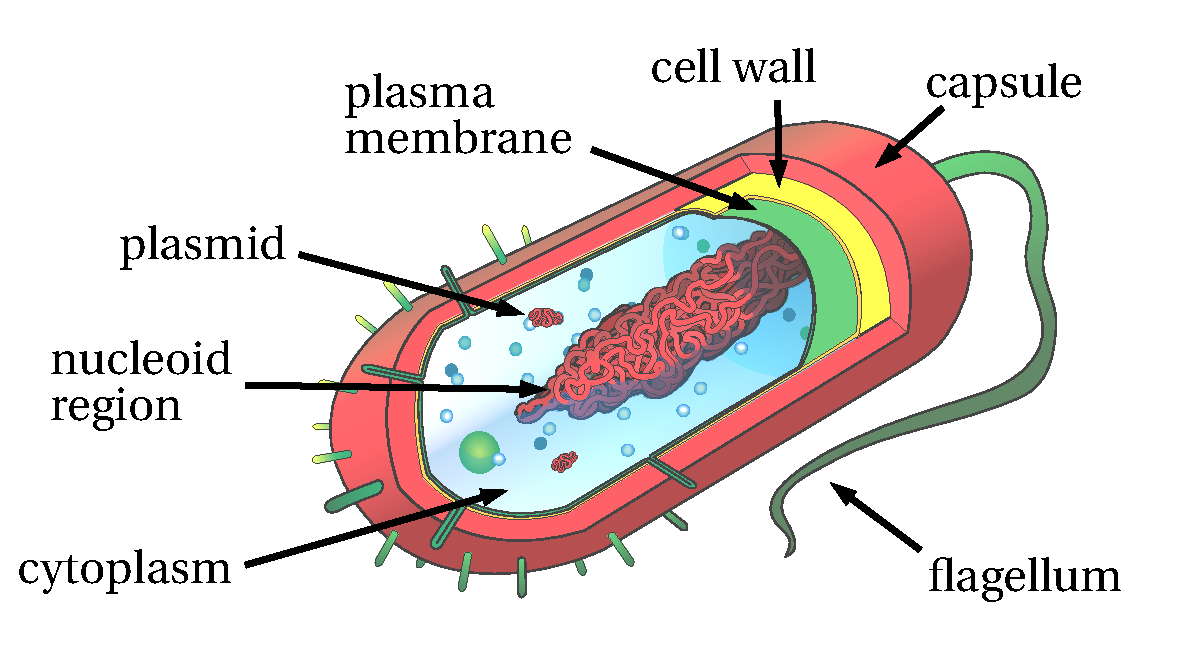
\includegraphics[width=0.8\linewidth]{Theory/Pics/bacteria}
	\caption{Basic structure of bacteria cell. Adapted from \textcite{Villarreal2008} and \textcite{Mader1998}.}
	\label{fig:bacteria}
\end{figure}



Bacteria are morphologically diverse and can appear spherical, rod-shaped, spiralled or filamentous \parencite{Wang2009}. Cell wall structure varies greatly among bacteria, with two major divisions being species with Gram-positive or Gram-negative walls \parencite{Rosenberg2013}. Both types have been identified in the battery recycling plant consortium: \textit{Enterococcus} and \textit{Clostridium} species are classified as Gram-positive, whereas \textit{Klebsiella} and \textit{Ralstonia} species are Gram-negative \parencite{Horstman2019,Peens2018}.

Gram-positive bacteria have a \SIrange[range-units = single]{20}{80}{\nano\meter} thick peptidoglycan (Figure~\ref{fig:peptidoglycan}) layer connected by amino acids and makes up \SIrange[range-units = single]{40}{90}{\percent} of the cell wall \parencite{Wang2009}. Teichoic acids link peptidoglycan to the plasma membrane. Functional groups within these two molecules as well as teichuronic acids contribute to an overall negative charge that facilitates the binding of metals \parencite{Vijayaraghavan2008}.

\begin{figure}[tbph!]
	\centering
	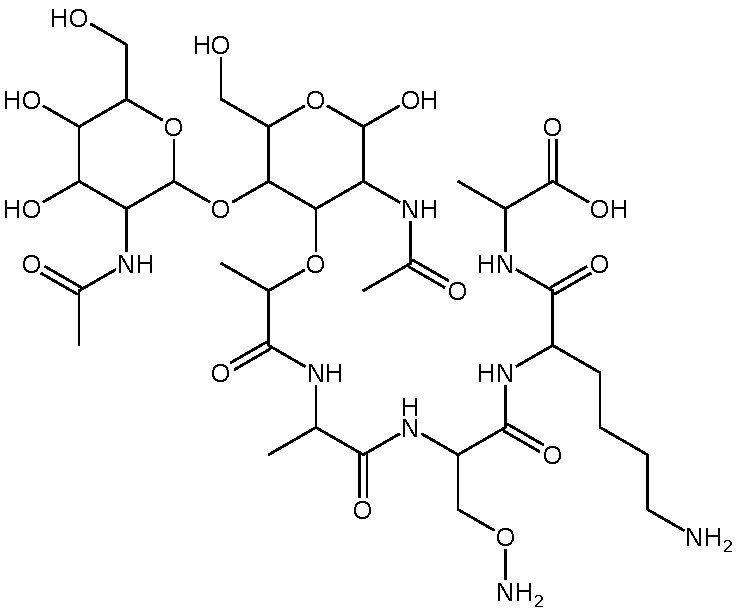
\includegraphics[width=0.7\linewidth]{Theory/Pics/peptidoglycan}
	\caption{Peptidoglycan monomer. Adapted from the \textcite{NCBI_pep}.}
	\label{fig:peptidoglycan}
\end{figure}

Gram-negative cell walls have significantly less peptidoglycan (\SIrange[range-units = single]{10}{20}{\percent} composition)  sandwiched between the plasma membrane and an outer membrane made up primarily of phospholipids and lipopolysaccharides \parencite{Vijayaraghavan2008}. Figure~\ref{fig:lps} presents a typical lipopolysaccharide. The functional groups in peptidoglycan, phospholipids and lipopolysaccharides are responsible for the anionic character  of the cell wall \parencite{Vijayaraghavan2008}.

\begin{figure}[tbph!]
	\centering
	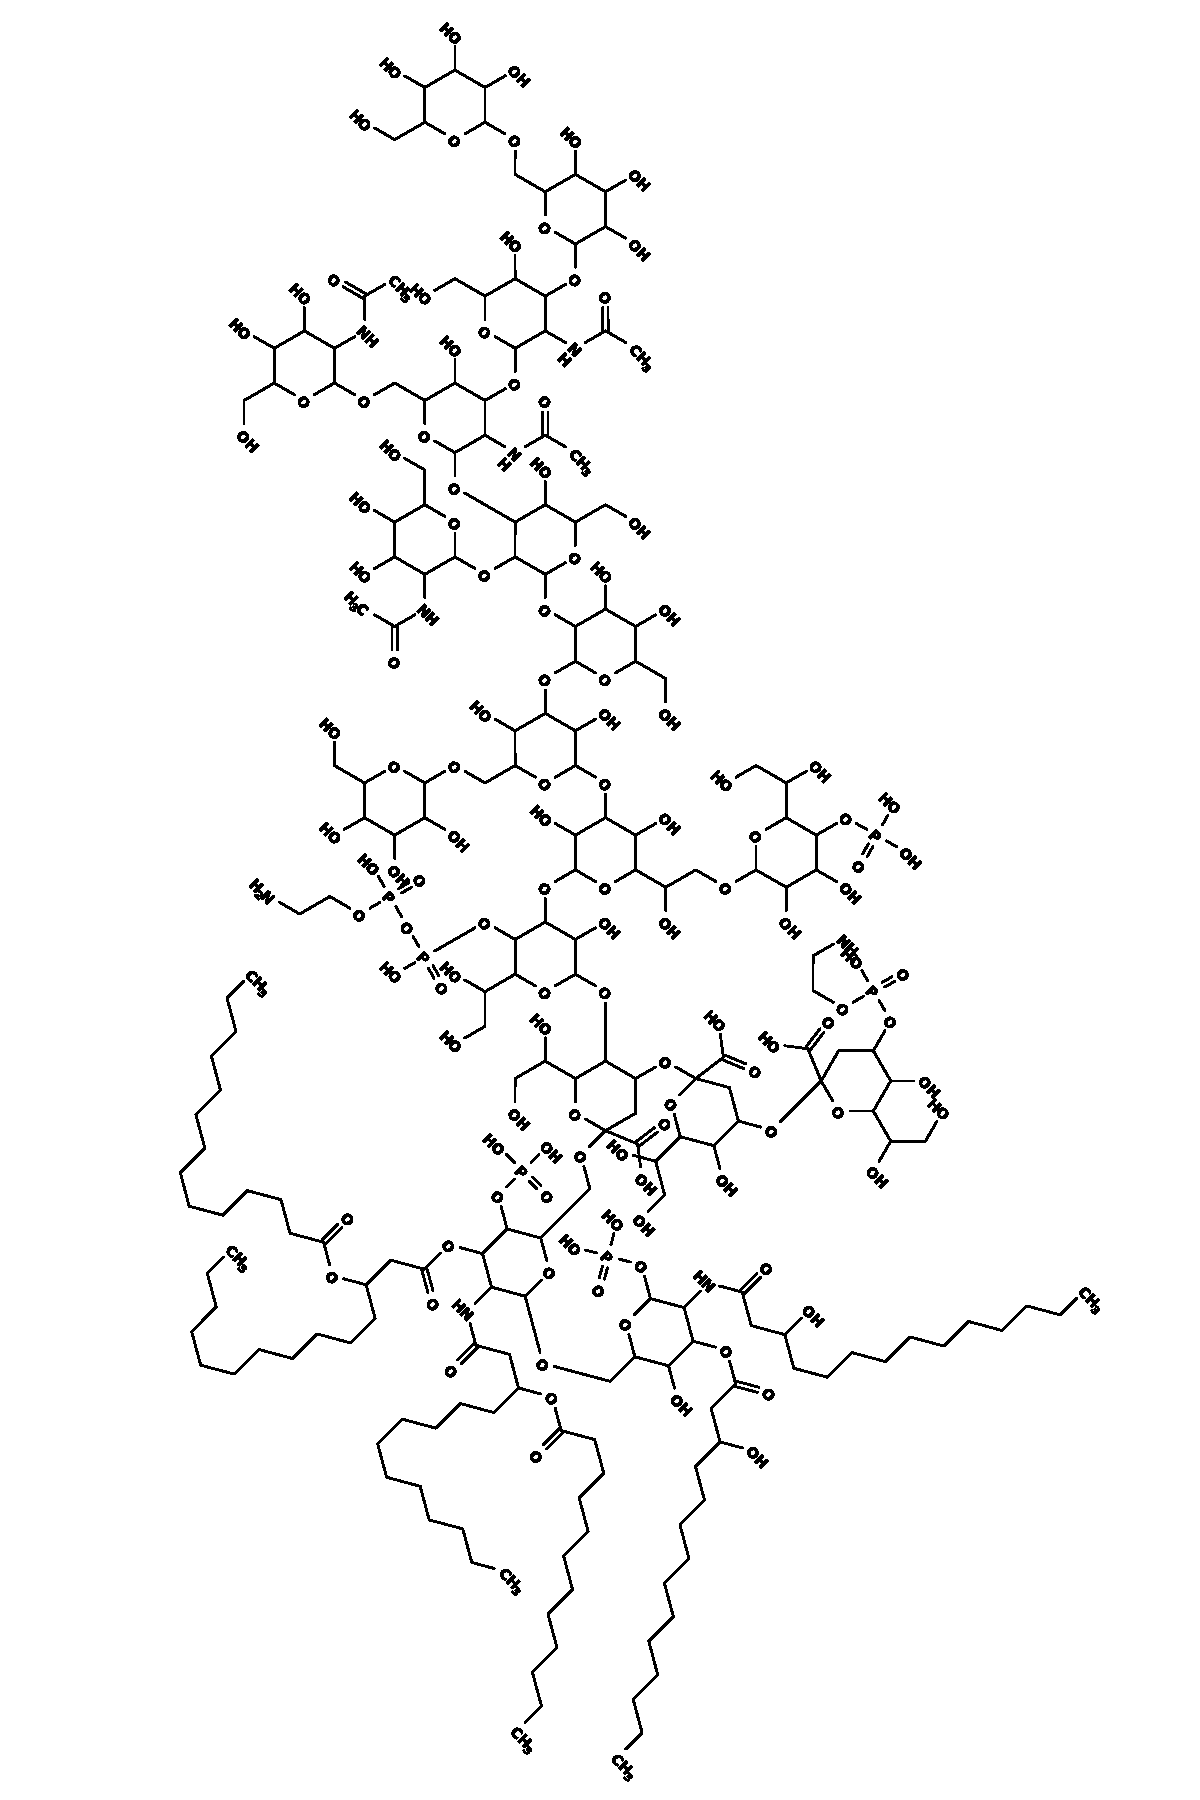
\includegraphics[width=0.9\linewidth]{Theory/Pics/lps}
	\caption{Example of a lipopolysaccharide molecule typically found in species like \textit{Escherichia coli} \parencite{Whitman2010}. Adapted from \textcite{NCIB_lps}.}
	\label{fig:lps}
\end{figure}



Extracellular polymeric substances (EPS) are also secreted on the surfaces of some bacteria and consist of proteins, polysaccharides, humic substances and nucleic acids \parencite{Zhang2017} that serve as both a protective layer and energy reserve for the cell \parencite{Liu2002}. These substances have been found to contain significant amounts of negatively charged functional groups \parencite{Wang2014}. Biofilms, capsules, slimes, and sheaths are composed of EPS and have been shown to contribute significantly to biosorption \parencite{Fomina2014}.

\subsubsection{Laboratory characterisation}

A variety of standard techniques are available for investigating and characterising the basic properties of an adsorbent. \textcite{Unuabonah2019} stresses the importance of accurate characterisation for the purposes of maximising adsorbent use in batch and continuous systems. Table~\ref{tab:techniques} outlines methods commonly used for determining adsorbent characteristics.

\setlength{\extrarowheight}{0.2cm}
\begin{small}
\begin{longtable}{>{\raggedright\arraybackslash}p{2.5cm}>{\raggedright\arraybackslash}p{3cm}p{7cm}}
	
	\caption{Techniques employed for determining various adsorbent properties. Adapted from \textcite{Tran2017}}
	\label{tab:techniques} \\

	
	\toprule
	Property  & Technique & Description \\
	\toprule
	\endhead
	
	\bottomrule
	\endfoot
	
	Surface chemistry & Energy dispersive  X-ray spectroscopy (EDS) & Samples are exposed to beam of X-rays, allowing elements to be identified as they excite and emit unique fluorescence X-rays.  \\ 
	& Fourier transform infrared spectroscopy (FTIR) & The amount of infrared light absorbed in a sample by molecular bonds is used to infer what bonds are present and how biosorption alters these bonds. \\ 
	& Raman spectroscopy (RS) & Visible or infrared light is is passed through a sample. The amount of light scattered can be used to identify molecular bonds. \\ 
	& Potentiometric titration & Point of zero charge (pH\textsubscript{pzc})  determined where there is an absence of adsorbent surface charge. \\ 
	& Electrophoresis & An electric field is applied in combination with light scattering to determine the zeta potential, defined as the potential difference at the interface of the diffusion layer of the adsorbent and bulk fluid used as a measure of electrostatic repulsion. \\ 
	
	Morphology & Scanning electron microscopy (SEM) & An electron beam scans across the adsorbent surface, resulting in scattered electrons that are used to generate an image. \\ 
	& Transmission electron microscope (TEM) & A high powered beams of electrons is sent through a cross section of a sample, resulting in interactions with the sample that are used to generate an image.  \\ 
	& Laser diffraction & Samples are exposed to a laser beam. The patterns of diffraction are analysed and used to infer particle size. \\ 

	Hydrophobicity & Water contact angle & The shape of the liquid-vapour interface of water on the sample is used to determine surface wettability. \\ 

	Textural property & BET specific surface area & The volume of \ce{N_2} adsorbed on the adsorbent surface can be used to infer surface are. \\ 

	Thermal stability & Thermal gravimetric analysis & The mass of a sample is recorded as a function of temperature and time to quantitatively analyse composition. \\ 

	Crystalline structure & X-ray diffraction & The diffraction pattern that arises from a sample being exposed to an X-ray beam is used to identify crystalline compounds. \\ 

	Proximate analysis & ASTM international standards & A variety of standardised methods employed to determine the distribution of major constituents. \\ 

	Ultimate analysis  & ASTM international standards & A variety of standardised methods employed to determine the distribution of carbon, hydrogen, oxygen and nitrogen. \\ 
	Adsorption of substance & Iodine number & The mass of iodine consumed by the adsorbent is used to compare adsorption surface area and porosity. \\ 
	& Molasses number & The measure of the amount of colour removed from molasses by an adsorbent and is used to evaluate the macro pore structure. \\ 
	& Methylene blue index & The measure of the amount of methylene blue adsorbed by a sample for the purpose of determining the cationic exchange capacity. \\
\end{longtable}
\end{small}

\subsection{Mechanisms of metal biosorption}

Biosorption mechanisms are highly complex and can involve multiple, simultaneous reactions that contribute to differing degrees \parencite{Fomina2014}. Figure~\ref{fig:sorption-mechansims} gives an overview of the mechanisms involved in biosorption within the context of sorption as a whole. However, the hierarchical arrangement of mechanisms differs among authors \parencite{Robalds2016}. The  extent to which each mechanism is involved varies significantly and is dependent on the adsorbate, ionic strength of solution and the chemical nature of the adsorbent \parencite{Yang2019}.

\begin{figure}[htbp!]
	\centering
	\begin{small}
	\begin{forest}
		for tree={
			draw,
			align=center
		},
		forked edges,
		[Sorption [Adsorption[Biosorption [Physisorption] [Ion exchange] [Chemisorption [Complexation (including coordination)] ]  [Microprecipitation]] [Other materials]] [Absorption]]
	\end{forest}
\end{small}
	\caption{Classification sorption mechanisms as proposed by \textcite{Robalds2016}}
	\label{fig:sorption-mechansims}
\end{figure}

\paragraph{Physisorption} Physical adsorption of ions onto biomass is primarily caused by van der Waals and electrostatic forces \parencite{Suzuki1990}. Due to the ionisation of functional groups, most biosorbents have been found to have net negative surface charges  \parencite{Farhan2015} that assist in the  attraction of positive metal ions towards the adsorbent \parencite{Hammaini2007}. 

\paragraph{Ion exchange} Light metal ion exchange involves several adsorption mechanisms where the cations \ce{Ca^2+}, \ce{Mg^2+}, \ce{K+}, and \ce{Na+} are released from the biomass surface and replaced by a heavy metal. Table  \ref{tab:th_vem} shows the molar ratio of \ce{Pb^2+} bound by adsorption to cations released as a result of adsorption, $R$\textsubscript{b/r}. If $R\textsubscript{b/r} \le 1$, then ion exchange is a prominent mechanism of adsorption. On the contrary, if $R\textsubscript{b/r} \ge 1$, then other mechanisms would dominate heavy metal adsorption \parencite{Saha2017}. It has also been reported that high concentrations of light earth metals tend to compete with heavy metals for adsorption sites adsorption \parencite{Xu2013}.

% \usepackage{array} is required
\begin{table}[htbp!]
\setlength{\extrarowheight}{0.3cm}
\centering
\caption{Contribution of cation exchange to \ce{Pb^2+} adsorption}
\label{tab:th_vem}
\begin{small}
\begin{tabular}{>{\raggedright\arraybackslash}m{3cm}>{\centering\arraybackslash}m{2cm}>{\centering\arraybackslash}m{2cm}m{3cm}}
	\hline 
	Biosorbent & Cations released & $R$\textsubscript{b/r} (mol \ce{Pb^2+}/mol cation)& Reference \\ 
	\hline 
	Sludge derived biochar & \ce{Mg^2+}, \ce{Ca^2+}, \ce{K^+}, \ce{Na^+} & 0.768 & \textcite{Lu2012} \\ 
	\textit{Colocasiaesculenta}(L.) Schott & \ce{Ca^2+, K+} & 0.12 & \textcite{Saha2017} \\ 
	\textit{Agaricus bisporus} & \ce{Mg^2+}, \ce{Ca^2+}, \ce{K^+} & 0.9382 & \textcite{Xu2013} \\ 
	\hline 
\end{tabular} 
\end{small}
\end{table}

\paragraph{Chemisortption} 

Functional group complexation is a category of adsorption mechanisms whereby ligands act as  binding sites by donating electron density to metal ions \parencite{Kotz2014,Smith2014}. This mechanism is initiated by the deprotonation of a ligand, as illustrated for divalent metals in Equation~\ref{eq:th_metalligand}, Equation~\ref{eq:th_metalligand1b} and Equation~\ref{eq:th_metalligand2}.
\begin{align}
\label{eq:th_metalligand}
	\ce{LH  &-> L- +  H+}\\
\label{eq:th_metalligand1b}
	\ce{L- + M^2+ &-> LM+}\\
\label{eq:th_metalligand2}
	\ce{2L- + M^2+ &-> 2LM}
\end{align}
Here, \ce{L} represents functional groups that act as ligands and \ce{M} represents the metal.  Functional group complexation can be a prominent adsorption mechanism for some bacteria that use it to concentrate terminal electron accepting ions on the cell wall surface \parencite{Haas2001}. The functional groups most prominently involved adsorption include hydroxyl and carboxyl groups \parencite{Lu2012,Chen2014,Costa2010,Fomina2014}. Biomass typically contains an abundance of these groups, as seen in Figure~\ref{fig:peptidoglycan} and Figure~\ref{fig:lps}. Other functional groups like phosphate, amine, carbonyl, and ether also play a role \parencite{Fein1997,Mathew2018,Chen2006}. The interaction between functional groups and aqueous metals involves a variety of arrangements that make modelling complexation problematic \parencite{Chen2006}, as demonstrated in Figure~\ref{fig:dentates} and Figure~\ref{fig:outersphere} for carboxyl groups. 

\begin{figure}[tbph!]
	\centering
	\schemestart
	{\small a) \chemfig{R-(=[1]O)-[7]OH} \quad b) \chemfig{R-(=[1]O)-[7]O\ce{M+}} \quad c) \chemfig{R-**[90,270,dash pattern=on 2pt off 2pt]4(-O-[,,,,dash pattern=on 2pt off 2pt]\ce{M}-[,,,,dash pattern=on 2pt off 2pt]O-)}\quad d) \chemfig{R-(-[1]O\ce{M+})-[7]O\ce{M+}}}
	\schemestop
	\caption{Possible inner-sphere functional group complexation with a divalent metal \ce{M^2+} and carboxyl groups, with a) being protonated before complexation, b) unidentate complexation, c) bindentate complexation, and d) bridging. Adapted from \textcite{Chen2006}.}
	\label{fig:dentates}
\end{figure}


\begin{figure}[tbph!]
	\centering
	\schemestart
	{\small
	\chemfig{R-(=[1]O)-[7]\ce{O-}-[,,,,dash pattern=on 2pt off 2pt]
		H_2O-[,,,,dash pattern=on 2pt off 2pt] \ce{M^2+}
		([:90]-[,,,,dash pattern=on 2pt off 2pt]O([:90,0.5]-H|_2))
		([:-90]-[,,,,dash pattern=on 2pt off 2pt]O([:-90,0.5]-H|_2))
		-[,,,,dash pattern=on 2pt off 2pt]OH_2
	}}
	\schemestop
	\caption{Possible outer-sphere complexation with divalent metal \ce{M^2+} and a carboxyl group. Adapted from \textcite{Worch2012}.}
	\label{fig:outersphere}
\end{figure}



\parencite{Ngwenya2015}



Due to the role of deprotonation, solution pH has a large impact on functional group complexation \parencite{Lee1999,Chen2014,Worch2012}. At lower pH values, \ce{H+} ions compete with metals for adsorption sites \parencite{Hammaini2007} while at higher pH values divalent metals form aqueous hydroxide species \parencite{Grive2010}. Optimal pH values between 4 and 6 frequently reported in biosorbent studies \parencite{DuncanJ.R.2003,Chen2006,Costa2010,Guiza2017,Hammaini2007,Lu2012}. 

The role of outer sphere complexation can be investigated by experimentation, since it is more sensitive to variations in ionic strength than inner sphere complexation \parencite{Ngwenya2015}.The extent to which each functional group participates in biosorption can also be investigated by experiment. Esterification of hydroxyl  and carboxyl groups by acidic methanol, for example, is capable of blocking the complexation of these functional groups. This process has been found to reduce \ce{Pb(II)} biosorption by up to \SI{38}{\percent} in apple residue \parencite{Lee1999} and up to  \SI{42}{\percent} in sludge derived biochar \parencite{Lu2012}. 

Potentiometric titration is also used to determine the equilibrium constants and concentration of various functional groups \parencite{Turner2005}, while Boehm titrations can be used to identify and quantify carboxylic, lactonic, and phenolic functional groups \parencite{SeungKim2016}.

\paragraph{Microprecipitation}  The surface precipitation of \ce{Pb(II)} generally involves reactions with phosphate to form pyromorphite and  hydropyromorphite \parencite{Li2017}.

\subsection{Modelling batch adsorption}

The employment of biosorption models prove useful in gaining an understanding of adsorbent capacity, the mechanisms of adsorption, the influence of operating conditions, equilibrium behaviour and optimisation possibilities \parencite{Anastopoulos2015,Unuabonah2019}. Modelling the process of biosorption has been undertaken using several approaches that are grouped as either empirical (equilibrium and kinetic) or mechanistic \parencite{Chen2006}. 

Empirical models  are not computationally intensive, and, as the name suggests are more focused on predicting the outcome of experimental results based on limited adjustable parameters \parencite{Vijayaraghavan2008}. Almost all empirical models are fit only  for specific temperature and pH operating conditions, although some authors have modified existing adsorption models to predict the effect of pH or temperature \parencite{Esposito2002,Jeppu2012}. The kinetic and equilibrium empirical models presented in this dissertation were not derived for biosorption nor do many of their assumptions apply, yet they have been shown as capable of reflecting biosorption experiments \parencite{Vijayaraghavan2008}.  

\subsubsection{Equilibrium models} 

Several empirical equilibrium models are given in Table~\ref{tab:emp_eq}.

Mechanistic models are based on the knowledge of binding sites from biomass characterisation and the associated adsorption reactions \parencite{Vijayaraghavan2008}. These models are used less often than empirical counterparts but are more valuable for explaining the outcome of experiments \parencite{Unuabonah2019}. The models presented in this section deal with describing surface complexation mechanism.

The following equilibrium equations can be used to describe acid-base chemistry and unidentate surface complexation at an oxidic binding site  \parencite{Ngwenya2003,Stumm1992}: 
\begin{align}
\label{eq:deprot}
\ce{R-OH^0+ &<=> R-O^- + H+}  & K_1= \ce{\frac{\{R-O^-\}$ a $ _{H}}{\{R-OH^0\}}} \\
\label{eq:prot}
\ce{R-OH2^+ &<=> R-OH^0 + H+}  & K_2= \ce{\frac{\{R-OH^0-\}$ a $ _{H}}{\{R-OH2^+\}}} \\
\label{eq:surfcomp}
\ce{R-O^- + M^{$m$+}  &<=> R-OM^{$m-1$}}  & K_M= \ce{\frac{\{R-OM^{$m-1$}\}}{\{R-O^-\} $ a $ _M }}
\end{align}
where \ce{R} represents the cell wall, \ce{M^{$m$+}} represents a metal ion of valence $ m $, and \ce{$ a_i $} is the activity the species $ i $. The notation $ \{\} $ denotes concentration in \si{\mol\per\gram} adsorbent, and can be converted to units of \si{\mol\per\liter} solution through multiplication with adsorbent concentration. The total metal concentration is defined as:
\begin{equation}
\label{eq:sitemassbal_met}
\ce{[M]}_\textrm{tot} = \ce{[M^{$m+$}] + [R-OM^{$m-1$}]} 
\end{equation}
Furthermore, the total number of sites can be found from the mass balance:
\begin{equation}
\label{eq:sitemassbal}
\ce{\{R-O\}}_\textrm{tot} = \ce{\{R-O^-\} + \{R-OH^0\} + \{R-OH2^+\} +\{R-OM^{$m-1$}\}} 
\end{equation}
Activity can be calculated using the Davies equation \parencite{Turner2005} as
\begin{align}
a_i &= c_i \gamma_i\\
\log\left(\gamma_i\right) &= -0.5092z^2 \left( \frac{\sqrt{I}}{1 + \sqrt{I}} - 0.3I\right)
\end{align}
where $ c_i $ is molar concentration in \si{\mole\per\liter}, $ \gamma_i $ is the activity coefficient, $ z $ is the ion valence, and  $ I $ is the ionic strength in \si{\mole\per\liter}.

The surface charge introduced by functional groups on adsorbents produces an electric field that interacts with aqueous ions. This influence on the equilibrium constant $ K_n $ for reaction $ n $ can be described as follows \parencite{Fein1997}:
\begin{equation}
K_n = K_{n,\mathrm{~int}} \exp\left(-\frac{\Delta zF\psi}{RT}\right)
\end{equation}
where $ K_{n,\textrm{~int}} $ is the equilibrium constant for reaction $ n $ when no surface charge is present, $ \Delta z $ is the change in valence for the surface species, $ F $ is the  Faraday constant (\SI{96485}{\coulomb\per\mole}), $ \psi $ is the surface potential in \si{\volt}, $ R $ is the gas constant in \si{\joule\per\mol\per\kelvin} and $ T $ is the temperature in \si{\kelvin}.

Several models have been developed for calculating $ \psi $ as a function of surface charge density to determine the influence of electrostatic effects on $ K_n $. Surface charge density is generally calculated using the sum of charged sites
\begin{equation}
\sigma = F\sum_j \left(\frac{\ce{\{R-O^-$_j$\} + \{R-OH2^+$_j$\}}}{A_{m}}\right)
\end{equation}
where $ j $ is a specific functional group, $ \sigma $ is surface charge density in \si{\coulomb\per\meter\squared},  $ A_{m} $ is the specific surface area in \si{\meter\squared\per\gram}. Potentiometric titration experiments can also be used to determine $ \sigma $:
\begin{align}
\sigma &= \frac{Q_sF}{A_m}\\
Q_s &= \frac{V}{W} \left( c_a - c_b - \log\left(\textrm{pH}\right) + \log\left(\textrm{pOH}\right) \right)
\end{align} 
Here, $ Q_s $ is the surface charge calculated from titration in \si{\mole\per\gram} adsorbent, $ V $ is the volume of adsorbate-bearing solution in \si{\liter}, $ W $ is the dry mass of adsorbent in \si{\milli\gram}, and $ c $ is the concentration in \si{\mol\per\liter} of acid $ a $ or base $ b $ added during titration.

Four of models used to describe the effect of $ \sigma $ on $ \psi $ are discussed in this section.



\paragraph{Non-electrostatic adsorption} In order to simplify surface complexation modelling, $ K_n = K_{n,\mathrm{~int}} $ is assumed in the non-electrostatic adsorption model (NEM) \parencite{Turner2005}. \textcite{Esposito2002} employed a simple mechanistic NEM for modelling heavy metal adsorption onto the bacteria \textit{Sphaerotilus natans}. The model assumes an ideal solution, negligible electrostatic effects, a non-competitive mechanism and only one type of binding site. The assumptions result in the following relationships:
\begin{align}
K_1 &= K_{1,\textrm{~int}} \\
K_M &= K_{M,\textrm{~int}} \\
\ce{\{R-OM^{$m-1$}\}} &= \frac{q_e}{M_\textsubscript{M}}   \\
\ce{$a$_M &= [M^{$m$+}]} = c_e \\
\ce{$a$_H &= [H^+]} = 10^{-\textrm{pH}} 
\end{align}
Where $ M_\textsubscript{M} $ is the molar mass of metal M. These equations can be combined with the equilibrium constants of Equation~\ref{eq:deprot} and Equation~\ref{eq:surfcomp} as well as the mass balance of Equation~\ref{eq:sitemassbal} to derive the isothermal profile:
\begin{equation}
q_e = \frac{c_e M_\textsubscript{M}\ce{\{R-O\}}_\textrm{tot}} {\left(1 + 10^{-\textrm{pH}}/K_1\right) \left(K_M + c_e\right)}
\end{equation}

\paragraph{Constant capacitance} The constant capacitance model is used under the assumption that only inner-sphere complexes form, no surface complexes are formed with ions from the background electrolyte, and that the suface has only one plane of charge \parencite{Goldberg1995}. The surface potential $ \psi $ is determined with the expression \parencite{Ngwenya2003}
\begin{equation}
\psi = \frac{\sigma}{C}
\end{equation}
$ C $ is capacitance density in \si{\farad\per\meter\squared}. \textcite{Fein1997} found that a $ C $ of \SI{8.0}{\farad\per\meter\squared} best fit titration data for \textit{Bacillus subtilis}. Other authors have subsequently made use of this capacitance density for modelling \textit{Pantoea agglomerans} \parencite{Ngwenya2009}, \textit{Escherichia coli} \parencite{Chang2020}, and a culture sourced from diesel contaminated soil \parencite{Ngwenya2003}. Parameter optimisation is, however, relatively insensitive to the chosen value of $ C $ \parencite{Lutzenkirchen1999}.

\paragraph{Double layer}

The double, diffuse, or diffuse double layer model has the same assumptions as the constant capacitance model with the exception of having two planes of charge \parencite{Goldberg1995}. The relationship between surface potential and surface charge density is described as \parencite{Turner2005}
\begin{equation}
\psi = \frac{2RT}{zF} \sinh^{-1} \left( \frac{\sigma}{\sqrt{8RT\epsilon\epsilon_0c}} \right)
\end{equation}
Here, $ z $ is the counter ion valence, $ c $ is the concentration of the counter ion in \si{\mole\per\liter}, $ \epsilon $ is the dielectric constant of water (78.5), and $ \epsilon_0 $ is the permittivity in vacuum (\SI{8.854e-12}{\coulomb\per\volt\per\meter}) \parencite{Huang2014}. 

\paragraph{Donnan shell} \textcite{Ohshima1990} remark that the double layer model is only accurate for ion-impenetrable surfaces and should not be applied to cell walls as a result. A more suitable complexation model is therefore given as \parencite{Ohshima1990, Turner2005}:
\begin{align}
\psi_\textrm{DON} &= \frac{RT}{zF} \sinh^{-1} \left( \frac{\sigma_s}{2zFc} \right)\\
\psi &= \psi_\textrm{DON} - \frac{RT}{zF} \tanh \left(\frac{zF \psi_\textrm{DON}}{2RT}\right)
\end{align}
where $ \psi_\textrm{DON} $ is the Donnan potential in \si{\volt}. This model differs from the double layer and constant capacity models in that volume charge density ($ \sigma_s $ in \si{\coulomb\per\meter\cubed}) is used instead of $ \sigma $. This is calculated as
\begin{equation}
\sigma_s = F\sum_j \left(\frac{\ce{\{R-O^-$_j$\} + \{R-OH2^+$_j$\}}}{V_m}\right)
\end{equation}
Here, $ V_m $ is the specific volume of the adsorbent shell or the Donnan volume in \si{\meter\cubed\per\gram}. \textcite{Yee2004} calculates $ V_m $ using a dry cell density of \SI{6.7e12}{\cell\per\gram} and cell wall volume of \SI{1.12}{\micro\meter\cubed\per\cell} for \textit{Bacillus subtilis}. The cell wall volume was calculated on the basis of a cell wall thickness of \SI{25}{\nano\meter} and cylindrical cell geometry with dimensions of 1 $ \times $ \SI{5}{\micro\meter}, although \textcite{Yee2004} caution that cell wall charge is highly sensitive to cell dimension and density estimates. 

More complicated mechanistic models have been developed to factor in multiple types of binding sites \parencite{Pagnanelli2005}, metal hydrolysis equilibria \parencite{Yang1999,Haas2001,Dai2010} and the influence of alkaline earth metal concentration \parencite{Chen2006}. These additional factors often require further experimentation and solving of multiple, complex non-linear equations which limit their implementation \parencite{Vijayaraghavan2008}.

\paragraph{Thermodynamics} Many authors make use of adsorption isotherms at multiple temperatures to investigate the spontaneity, randomness and the exothermic or endothermic nature of biosorption \parencite{Rangabhashiyam2019}. Equation~\ref{eq:td1} and Equation~\ref{eq:td2} are used for this purpose:
\begin{align}
\Delta G^\circ &= -RT \ln K_C \label{eq:td1}\\
\ln K_C &= \frac{-\Delta H^\circ}{RT} + \frac{\Delta S^\circ}{R} \label{eq:td2}
\end{align}
where $ \Delta G^\circ $ is the change in Gibbs free energy  (\si{\joule\per\mole}), $ \Delta H^\circ $ is the change in enthalpy  (\si{\joule\per\mole}) and $ \Delta S^\circ $ is the change in entropy (\si{\joule\per\mole\per\kelvin}). $ T $ is the temperature (\si{K}), $ R $ is the universal gas constant, and $ K_C $ is the distribution coefficient calculated as $ K_C = q_e/C_e $.


\newgeometry{left=1cm,right=1cm,bottom=2cm,top=1cm}
\begin{landscape}
	\setlength{\extrarowheight}{0.2cm}
	\begin{footnotesize}
		\begin{longtable}{>{\raggedright\arraybackslash}p{2cm}p{7.25cm}p{4.5cm}p{7.25cm}}
			
			\caption{Empirical equilibrium adsorption models}
			\label{tab:emp_eq} \\
			
			
			\toprule
			Model  & Description & Equation & Description of equation  \\
			\toprule
			\endhead
			
			\bottomrule
			\endfoot
			
			Langmuir 
			
			& The Langmuir adsorption isotherm model is the most frequently encountered equilibrium model in literature. It was originally developed for the adsorption of gases onto surfaces and is used under the assumption that there is a fixed number of homogeneous sites where reversible, monolayer adsorption takes place with no interaction between adsorbate species \parencite{Langmuir1918}. 
			
			& \begin{align}
			q_e=\frac{q_{\mathrm{max}}K_LC_e}{1+K_LC_e} \label{eq:Lang}
			\end{align} 
			
			& $q_e$ is the equilibrium adsorption capacity (\si{\milli\gram\per\gram}), $q_{\mathrm{max}}$ is the maximum adsorption capacity (\si{\milli\gram\per\gram}), $K_L$ is the Langmuir adsorption equilibrium constant (\si{\liter\per\milli\gram}) related to affinity between adsorbate and adsorbent, and $C_e$ is the equilibrium concentration of adsorbate in solution (\si{\milli\gram\per\liter}). Heterogeneous adsorption can be modelled with the sum of multiple homogeneous isotherms \parencite{Langmuir1918}. \\
			
		
			Modified Langmuir
			
			& \textcite{Esposito2002} proposed a modification for Equation~\ref{eq:Lang} that describes the effect of pH on $ q_\mathrm{max} $.
			
			& \begin{equation}
			q_\mathrm{max} = \frac{q_0e^{k_E \text{pH}}}{1 - \dfrac{q_0}{q_\infty} \left( 1-e^{k_E \text{pH}}\right)}
			\end{equation} 
			
			& $ q_0 $, $ q_\infty $, and $ k_E $ are adjustable constants. \\
			
			
			
			Freundlich
			
			& The Freundlich isotherm equation describes reversible, non-ideal, multilayer adsorption and is usually used for heterogenous adsorbents like biomass \parencite{Foo2010}. This model has, however, been found to inadequately describe the linearity range at very low concentrations or saturation effects at very high concentrations \parencite{Tran2017}.
			
			& \begin{align}
			q_e=K_FC_e^\alpha \label{eq:freund}
			\end{align}
			
			& $K_F$ is the Freundlich constant in (\si{\milli\gram\per\gram})(\si{\milli\gram\per\liter})$^{-\alpha}$ and $\alpha$  is the Freundlich intensity parameter. The isotherm is linear when $\alpha=1$, favourable when $\alpha \le 1$, and unfavourable when $\alpha \ge 1$ \parencite{Tran2017}. In addition, it has been reported that a value for $\alpha$ between 0 and 1 indicate surface heterogeneity,  with more heterogeneous surfaces having values closer to 0 \parencite{Foo2010}. \\
			
			Sips
			
			& The Sips isotherm, also referred to as the Langmuir-Freundlich  model \parencite{Jeppu2012}, is a three parameter power function based the assumption of continuously distributed affinity coefficients \parencite{Bolster2007a}. The Sips isotherm has been found to predict adsorption involving the occupation of two sites by a single adsorbent \parencite{Chan2012}. 
			
			& \begin{align}
			q_e=\frac{q_{\mathrm{max}}K_{S}C_e^s}{1+K_{S}C_e^s} \label{eq:sips}
			\end{align}
			
			& $K_{S}$ is the Sips constant in (L/mg)$^s$ and $s$ is a fitting parameter between 0 and 1. Similar to the Freundlich model, this isotherm is appropriate for heterogeneous surfaces. At high adsorbate concentrations the model reduces to the Langmuir isotherm (Equation \ref{eq:Lang}) and at low concentrations it resembles multilayer adsorption found in the Freundlich isotherm \parencite{Ayawei2017}. \\
			
			Modified Sips 
			
			& \textcite{Jeppu2012} proposed a modification for Equation~\ref{eq:sips} to account for the effect of pH on $ K_S $.
			
			&\begin{align}
			\log  K_{S} = M_1 \text{pH} + M_2
			\end{align}
			
			& $ M_1 $ and $ M_2 $ are constants. \\
			
			Redlich-Peterson
			
			& The Redlich-Peterson model is also described as a hybrid between the Langmuir and Freundlich isotherms \parencite{Ayawei2017}. This isotherm follows multilayer adsorption \parencite{Chan2012} and does not have good asymptotic behaviour for high adsorbate concentrations \parencite{Brouers2015}. 
			
			& \begin{align}
			q_e = \frac{K_{RP} C_e}{1 + a_{RP} C_e^r} \label{eq:rp}
			\end{align}
			
			&  $ K_{RP} $ is  a constant (\si{\liter\per\gram}), $ a_{RP} $ is a constant (\si{\liter\per\milli\gram})$^{-r}$ and $ r $ is a parameter with values constrained between 0 and 1. When $ r =1$, then Equation~\ref{eq:rp} reduces to the Langmuir isotherm (Equation \ref{eq:Lang}). At high concentrations of adsorbate, the Redlich-Peterson model reduces to the Freundlich isotherm (Equation \ref{eq:freund}). When $ r = 0 $, Equation~\ref{eq:rp} reduces to Henry's law \parencite{Ayawei2017}. \\
			
			Temkin
			
			& The Temkin adsorption isotherm focuses on adsorbent-adsorbate interactions. The model assumes a uniform distribution of heterogeneous binding energies and a linear decrease in heat of adsorption \parencite{Dada2012}.
			
			& \begin{equation}
			q_e = \frac{RT}{b_T} \ln \left(A_T C_e \right)
			\end{equation}
			
			& $ A_T $ is the Temkin isotherm equilibrium binding constant (\si{\liter\per\gram}), $ b_T $ is the Temkin isotherm constant (\si{\joule\per\mole}), and $ R $ is the universal gas constant of \SI{8.314}{\joule\per\mole\per\kelvin}. \\
			
			Dubinin-Radushkevich
			
			& This model assumes a Gaussian energy distribution of heterogeneous sites \parencite{Inyinbor2016}.
			
			& {\begin{align}
				q_e &= q_\textrm{max} e^{-K_{DR} \varepsilon^2} \\
				\varepsilon &= RT \ln \left(1 + \frac{1}{C_e}\right)
				\end{align}}
			
			& $ K_{DR} $ is the Dubinin-Radushkevich isotherm constant   (\si{\mole\squared\per\joule\squared}). \\
		\end{longtable}
	\end{footnotesize}
\end{landscape}
\restoregeometry

\subsubsection{Kinetic models} 

The modelling of time progress in adsorption can provide insight into the mechanism of sorption and behaviour leading up to equilibrium. Adsorption kinetics concerns four stages of transport \parencite{Worch2012}:
\begin{enumerate}
	\item Transport of adsorbate from bulk liquid phase to the stagnant boundary layer around the adsorbent.
	\item External diffusion of adsorbate through the stagnant boundary layer to the adsorbent surface.
	\item Internal or intraparticle diffusion of adsorbate. 
	\item Binding of adsorbate to final adsorption site.
\end{enumerate}
\textcite{Worch2012} further states that these steps are modelled under the assumptions that temperature is constant, the bulk solution is completely mixed, and that the adsorbent particle is spherical and isotropic. In most cases the first and final steps are fastest, thereby leaving the external and internal mass transfer as the rate limiting steps. Internal mass transfer includes both surface and pore diffusion, where surface diffusion is generally assumed to be the dominant step \parencite{Worch2012}. Several mass transfer and adsorbate binding models are given in this section, with empirical models presented in Table~\ref{tab:emp_kn}.

\paragraph{External diffusion} Fick's law of  diffusion can be used to model external mass transfer. However, this step is dependent on stirring speeds or flow rates and is almost never rate-limiting in experimental runs. As a result, it is generally not modelled by authors. 

\paragraph{Internal diffusion} Within a spherical adsorbent with a radius $ r $ (\si{\meter}) and effective adsorbate diffusivity $ D_e $ (\si{\meter\squared\per\second}), internal mass transfer can be described in Equation~\ref{eq:diff} \parencite{Largitte2016}:
\begin{align}
	\frac{\partial q}{\partial t} = \frac{D_e}{r^2} \frac{\partial}{\partial r} \left( \frac{r^2 \partial q}{\partial r} \right) \label{eq:diff}
\end{align}
Here, $ t $ denotes time (\si{\minute}). Integrated solutions to Equation~\ref{eq:diff} are given by \parencite{Boyd1947} and \parencite{Reichenberg1953} in Table~\ref{tab:emp_kn}  as Equation~\ref{eq:boyd} and Equation~\ref{eq:reichenberg} respectively. 

The Weber and Morris internal diffusion model is comparatively simpler and is also presented in Table~\ref{tab:emp_kn} as Equation~\ref{eq:wm1}.


\paragraph{Final adsorption}For the binding of an adsorbate to the final adsorption site, Langmuir kinetics consider the elementary reaction of metal \ce{M} adsorbing onto site \ce{S} as follows \parencite{Fogler2006}:
\begin{equation}
\ce{M + S <=> MS}
\end{equation}
The rate of adsorption $ r_a $ and the rate of desorption $ r_d $ is given in Equation~\ref{eq:ads} and Equation~\ref{eq:des} respectively:
\begin{align}
r_a &= k_aC(1 - \theta) \label{eq:ads} \\
r_d &= k_d \theta \label{eq:des}
\end{align}
Where $ k_a $ and $ k_d $ are rate rate constants for adsorption and desorption and $ \theta $ is the fraction of adsorption sites covered ($ 0 \le \theta \le 1 $). Therefore, the combined rate equation can be taken as:
\begin{align}
	\frac{d\theta}{dt} &= r_a - r_d\\
	\frac{d\theta}{dt}&= k_aC(1 - \theta) - k_d \theta \label{eq:lang-rate-theta}
\end{align}
If the grams of solute adsorbed at any time can be represented as a fraction of the equilibrium adsorption $ q_e $, i.e.\  $q =  q_e \theta$, then Equation~\ref{eq:lang-rate-theta} can be rewritten as:
\begin{align}
	\frac{dq}{dt}&= k_aC(q_e - q) - k_d q \label{eq:lang-rate-q}
\end{align}
Equation~\ref{eq:lang-rate-q} is also referred to as the Adam-Bohart-Thomas model \parencite{Zhao2011}. Defining $ K_L = k_a/k_d $,  Equation~\ref{eq:lang-rate-q} reduces to the Langmuir isotherm (Equation~\ref{eq:Lang}) at equilibrium. The integrated solution of Equation~\ref{eq:lang-rate-q} is given in Table~\ref{tab:emp_kn} as Equation~\ref{eq:psuedo-lang}. 

Pseudo-first- and pseudo-second-order models of kinetic adsorption have been developed and are also presented in Table~\ref{tab:emp_kn}. These models follow assumptions used to describe Langmuir adsorption \parencite{Largitte2016,Ho2000}. \textcite{Azizian2004} showed that the pseudo-first- and pseudo-second-order models could be derived from Langmuir kinetics presented in Equation~\ref{eq:lang-rate-theta}.  When the initial concentration of adsorbate $ C_0 $ is very high, or the process modelled is still in initial adsorption phases, or when relatively few binding sites are present on the adsorbent, then pseudo-first-order kinetics approximate Langmuir kinetics. Similarly, it was shown that the pseudo-second-order model can be derived from Langmuir kinetics when $ C_0 $ is relatively low, adsorption is at the final stage, or if active sites are relatively abundant on the adsorbent  \parencite{Wang2020}. 


\textcite{Stumm1992} presented a mechanistic approach to adsorption of divalent metal ions onto hydrous oxide surfaces. The process assumes attachment to the surface as an outer-sphere complex, followed by surface diffusion, metal complex dewatering, and finally the formation of a bond with the active site as follows:

\begin{align}
	\ce{R-OH + M(H2O)^2+_n &<=>[{$K$_{OS} }] R-OH \bond{...}M(H2O)^2+_n}\\
	\label{eq:dewater}
	\ce{R-OH \bond{...}M(H2O)^2+_n &->[{$k$_{ads} }]  \chemfig{R-O(-[1]H)-[7]{M(H2O)^{2+}_{\textit{n}-1}}} + H2O} \\
	\ce{ \chemfig{R-O(-[1]H)-[7]{M(H2O)^{2+}_{\textit{n}-1}}} &->[{$k$_{fast}}] R-O-M(H2O)^{+}_{n-1} + H+}
\end{align}
Here, $K_\textrm{OS}$ is the outer-sphere surface complex formation constant and is calculated as:
\begin{align}
	K_\textrm{OS} = \exp\left( -\frac{Z\psi}{RT}\right)
\end{align}
Additionally, $ k_\textrm{ads} $ is the intrinsic adsorption rate constant at zero surface charge. The magnitude of this constant is largely dependent on the rate of dewatering from the metal held in the outer-sphere complex (Equation~\ref{eq:dewater}). Assuming $k_\textrm{fast} >> k_\textrm{ads}$, the surface complex rate of formation is calculated as:
\begin{align}
	\frac{d[\ce{R-OM+}]}{dt} = K_\textrm{OS}k_\textrm{ads} \ce{[M^2+][R-OH]}
\end{align}

\newgeometry{left=1cm,right=1cm,bottom=2cm,top=1cm}
\begin{landscape}
	\setlength{\extrarowheight}{0.2cm}
	\begin{footnotesize}
		\begin{longtable}{>{\raggedright\arraybackslash}p{2cm}p{6cm}p{6cm}p{7.25cm}}
			
			\caption{Empirical kinetic adsorption models}
			\label{tab:emp_kn} \\
			
			
			\toprule
			Model  & Description & Equation & Description of equation  \\
			\toprule
			\endhead
			
			\bottomrule
			\endfoot
			
			Boyd
			
			&\textcite{Boyd1947} obtained an expression for Equation~\ref{eq:diff} to calculate the fractional attainment of adsorption equilibrium $ F $ as a function of time.
			
			& \begin{align}
			F = 1 - \frac{6}{\pi^2} \sum_{n=1}^\infty  \frac{1}{n^2} \exp \left( - n^2Bt \right) \label{eq:boyd}
			\end{align}  
			
			& $F = \cfrac{q}{q_e}$ and $B = \cfrac{\pi^2 D_e}{r^2}$. \\
			
			
			Reichenberg
			
			& A piecewise approximation for solving Equation~\ref{eq:boyd} derived by \textcite{Reichenberg1953} for long and short times.
					
			& {\begin{equation}
			Bt = 
			\begin{cases}
			2\pi - \dfrac{\pi^2F}{3} - 2\pi \sqrt{ 1 - \dfrac{\pi F}{3}} \\ \quad\quad\quad\quad\quad\quad F \le 0.85 \\
			-0.4977 - \ln\left(1-F \right) \\
			\quad\quad\quad\quad\quad\quad F > 0.85
			\end{cases} \label{eq:reichenberg}
			\end{equation}} 
		
			& With $ F $ being determined by experimental procedure, Equation~\ref{eq:reichenberg} can be used to solve for $ Bt $ and plotted as a function of $ t $. If internal mass transfer is the limiting rate, then the plot should be linear with segments of slope $ B $ that can be used to solve for effective diffusivity \parencite{El-Khaiary2011}.	\\
			
			Weber and Morris
			
			& Internal diffusion is frequently analysed in literature using the Weber and Morris model.
			
			& 
			{\begin{align}
			q & = k_{WM} t^{1/2} + c \label{eq:wm1} \\
			k_{WM} & = 6 \frac{q_e}{r}\sqrt{\frac{D_e}{\pi}} \label{eq:wm2}
			\end{align}}
			
			& $ k_{WM} $ is the diffusion rate constant and $ c $ is a constant \parencite{Largitte2016}. If $ q $ is plotted as a function of the square root of time and a single straight line is produced with $ c = 0 $, then intraparticle diffusion is the limiting factor. If the plot is multi-linear, then multiple rate limiting steps are involved \parencite{Fierro2008}. The slopes of each segment in the plot correspond to $ k_{WM} $ and can be used to solve for $ D_e $ in Equation~\ref{eq:wm2} \parencite{Tsibranska2011}.  \\
			
			
			Langmuir
			
			& The integration of Equation~\ref{eq:lang-rate-q} given by \textcite{Largitte2016}.   
			
			& \begin{equation}
			q\left(t\right) = q_e \frac{k^\prime_a}{k^\prime_a + k_d} \left[ 1 - e^{-\left(k^\prime_a + k_d\right)t} \right] \label{eq:psuedo-lang}
			\end{equation}
			
			& $ k^\prime_a $ is a pseudo-rate constant representing $ k_aC $.	\\
			
			Pseudo-first-order
			
			& \textcite{Lagergren1898} derived a model following Langmuir adsorption assumptions \parencite{Largitte2016,Ho2000} but with the assumption of negligible desorption. 
			
			& \begin{equation}
			q\left(t\right) = q_e \left( 1 - e^{-k_1t} \right) \label{eq:pfo}
			\end{equation}
			
			& $ k_1 $ is the pseudo-first-order rate constant  (\si{\per\minute}). Kinetics of sites with different binding energies can be represented by fitting adsorption as the sum of multiple pseudo-first-order compartments \parencite{Cornelissen1997} \\
			
			Pseudo-second-order
			
			& The pseudo-second-order model was first developed by \textcite{Ho2000} to describe kinetics of divalent metal adsorption onto sites in competition with hydrogen ions:
			{\begin{align*}
			\ce{2S- + M^2+ &<-> MS2} \\
			\ce{2HS + M^2+ &<-> MS2 + 2H+}
			\end{align*}}
			
			& \begin{align}
			q\left(t\right)=\frac{q_e^2k_2t}{1+q_ek_2t} \label{eq:pso}
			\end{align}
			
			& $ k_2 $ is the pseudo-second-order rate constant (\si{\gram\per\milli\gram\per\minute}).  \\
			
			Elovich
			
			& The Elovich kinetic model is a thermodynamic derivation for molecular exchange adsorption which occurs on a heterogeneous surface with activation energy that increases as molecules are adsorbed \parencite{Wu2009,Wang2020}. 
			
			& \begin{equation}
			q(t) = \frac{1}{b} \ln \left( 1+abt\right) \label{eq:elovich-int}
			\end{equation}
			
			& $ a $ is the initial rate of chemisorption (\si{\milli\gram\per\gram\per\minute}). The significance of $ b $ (\si{\gram\per\milli\gram}) has a variety of descriptions among authors, including representing the deceleration of adsorption \parencite{McLintock1970}, the desorption constant \parencite{Tran2017}, and an indication of the number of sites available \parencite{Fierro2008}. \\
			

		\end{longtable}
	\end{footnotesize}
\end{landscape}
\restoregeometry



\subsubsection{Model comparison}

Several mathematical tools have been developed for the comparison of models fit to experimental data to determine which  model most accurately describes reality. 

\paragraph{Coefficient of determination} In many studies, the coefficient of determination $  R^2  $ is used for model comparison. It is calculated as \parencite{El-Khaiary2011}:
\begin{equation}
	R^2 = 1- \frac{SS_E}{SS_T} \label{eq:r2}
\end{equation}
Where $ SS_E $ is the residual sum of squares and $ SS_T $ is the total sum of squares. For a model fit to data points $ q $ with predicted values $ q\textsubscript{mod} $,
 $ SS_E $ and $ SS_T $ are given in Equation~\ref{eq:sse} and Equation~\ref{eq:sst} respectively.  
\begin{align}
	SS_E &= \sum_{i}\left(q_i - q_{\textrm{mod,}i}\right)^2 \label{eq:sse} \\
	SS_T &= \sum_{i} \left(q_i - \bar{q}\right)^2 \label{eq:sst}
\end{align}
Here $ \bar{q} $ denotes the mean value of $ q $. While $ R^2 $ helps determine the accuracy of fit for a model, it is widely discouraged to compare models using it \parencite{El-Khaiary2011,Motulsky2003,Montgomery2013}. This is because $ R^2 $ is sensitive to outliers, tends to increase with increases in the range of the independent variable, and it favours models with more parameters \parencite{El-Khaiary2011}. 

\paragraph{Akaike information criterion} This criterion, abbreviated as AIC was developed with the purpose of comparing models to determine which one would have the highest likelihood of being accurate \parencite{Akaike1974}. The criterion has been modified into the corrected AIC, or AIC\textsubscript{C}, to remove bias found in small sample sizes for non-linear regression \parencite{Hurvich1989}. The AIC\textsubscript{C} is expressed as \parencite{Bolster2007a}: 
\begin{equation}
	\text{AIC}\textsubscript{C} = n \ln \left( \frac{SS_E}{n } \right) +2\left( n_p + 1 \right) + \frac{2\left( n_p + 1 \right)\left( n_p + 2 \right)}{n - n_p - 2} \label{eq:aicc}
\end{equation}
Where $ n $ is the number of data points and $ n_p $ is the number of parameters. AIC\textsubscript{C} is not unitless, and therefore the criterion only gains meaning when compared to another criterion of the same units. When considering two models, the probability $ P $ that the second model is more accurate than the first is calculated using Equation~\ref{eq:delta} and Equation~\ref{eq:p} \parencite{Motulsky2003}:
\begin{align}
	\Delta &= \text{AIC}\textsubscript{C, 2} - \text{AIC}\textsubscript{C, 1} \label{eq:delta} \\
	P &= \frac{e^{-0.5 \Delta}}{1 + e^{-0.5\Delta}} \label{eq:p}
\end{align} 


	
	\chapter{Experimental}

\section{General experimental procedures}

\subsection{Biosorption material preparation}
\label{sec:innoc}

Cultures were prepared in sterile batch reactors using the B consortium. The \SI{100}{\milli\liter} growth suspension contained \SI{20}{\gram\per\liter} tryptone, \SI{10}{\gram\per\liter} yeast extract, and \SI{1.0}{\gram\per\liter} \ce{NaCl} \parencite{Horstmann2020}. Culture preparation was done in the absence of lead, but \SI{0.43}{\gram\per\liter} \ce{NaNO3} was added to ensure that bacteria were still provided with nitrates previously supplied from \ce{Pb(NO3)2} in experiments done by \textcite{Horstmann2020}. Batch reactors were purged with nitrogen for \SI{3}{\min} to ensure anaerobic conditions \parencite{Peens2018b} and left to grow in a shaker-incubator for \SI{24}{\hour}, \SI{35}{\degreeCelsius} and \SI{120}{rpm}. To successfully inhibit the microbial respiratory chain and ensure \ce{Pb(II)} removal through biosorption alone, the culture was exposed to \SI{50}{\milli M} of \ce{NaN3}  \parencite{Cabrol2017} for \SI{3}{\hour}.

\subsection{Dry mass measurement}

Following the \SI{24}{\hour} culture growth period described in Section~\ref{sec:innoc}, a portion of the living bacteria was centrifuged at \SI{9000}{rpm} for \SI{10}{\min} before being oven dried overnight at \SI{85}{\degreeCelsius} for weighing.

\subsection{Plate count}

Plate count growth medium was prepared in sterile conditions and consisted of \SI{15}{\gram\per\liter} agar, \SI{20}{\gram\per\liter} tryptone, \SI{10}{\gram\per\liter} yeast extract, and \SI{1.0}{\gram\per\liter} \ce{NaCl}. Following the \SI{24}{\hour} culture growth period described in Section~\ref{sec:innoc}, a portion of the living bacteria was serially diluted in ultrapure water to the desired concentration. \SI{0.1}{\milli\liter} of diluted solution was thereafter spread onto solid agar plates and incubated at \SI{35}{\degreeCelsius} for \SI{48}{\hour}.

\subsection{Pb(II) concentration measurement}

Samples to be used for Pb(II) removal were diluted with ultrapure water to concentrations between \SIrange[range-phrase=~and~]{0}{10}{\gram\per\liter}. Analysis was thereafter done with an atomic absorption spectrometer (Perkin Elmer AAnalyst 400, Waltham, Massachusetts).

\subsection{Metabolic activity measurement}

Metabolic activity was measured with 3-(4,5-dimethylthiazol-2-yl)-2,5-diphenyl tetrazolium bromide (MTT). MTT is a yellow dye which is reduced to formazan crystals by the dehydrogenase system of viable gram-negative bacterial cells. MTT solution was prepared using \SI{5}{\gram\per\liter} MTT in ultrapure water. 

For metabolic activity readings, filtered (\SI{0.45}{\micro\meter}) and unfiltered samples were diluted 4 times and mixed with MTT to form a \SI{10}{\percent} MTT solution. The solution was incubated for an hour, after which formazan crystals were dissolved by dimethyl sulfoxide. A spectrophotometer with light at 550 nm was used to measure light absorbed by solution and infer metabolic activity from the difference between filtered and unfiltered samples \parencite{Peens2018}. 

\newpage

\section{Effect of initial Pb(II) and biomass concentration on equilibrium Pb(II) concentration}

\subsection{Introduction}

This section served to assist in experimental planning by provding insight into expected adsorption capacity and Pb removal. Knowledge of the relationship between these three variables also assists in assessing optimum concentrations and efficiency for biosorption by the consortia.

\subsection{Materials and methods}

Dead bacteria culture was prepared as described in Section~\ref{sec:innoc} and thereafter dispensed in volumes ranging from \SIrange{0.2}{3.4}{\milli\liter} into serum bottles containing \SIrange{50}{450}{\mgpl} \ce{Pb(II)}. To retain the same ionic strength as growth culture, \SI{0.17}{M} \ce{NaNO3} was added into serum bottles.

Serum bottles were left for \SI{3}{\hour} before samples were taken from each reactor and filtered. \ce{Pb(II)} concentration and metabolic activity were measured at the beginning and at equilibrium.


\subsection{Results and discussion}

Metabolic activity was undetected at the experiment initialisation and equilibrium, indicating successful inhibition of microbial activity by \ce{NaN3}.

Figure~\ref{fig:conc-vs-rem} (a) shows a clear increase in Pb(II) removal with higher biomass concentrations. This effect becomes less pronounced as biomass increases, and suggests that increments beyond \SI{47.5}{\mgpl} may lead to insignificant increases in lead removal. The decrease in adsorption efficiency with an increase in biomass is likely caused by a screen effect, where higher cell densities result in the blocking of active sites \parencite{Hammaini2007}. The range studied also shows peak lead removal at initial concentrations around \SI{130}{\milli\gram\per\liter} lead, regardless of how much biomass is present.

Figure~\ref{fig:conc-vs-rem} (b) illustrates how adsorption capacities of all biosorption concentrations fall on the same isotherm with a $q_\textrm{max}$ of around \SI{2700}{\mgg}. The cluster of low adsorption capacities at $C_e > \SI{200}{\mgg}$ is likely caused by errors introduced by dilutions, as a decrease in adsorption capacity with as $C_e$ increases does not fit a known isotherm type \parencite{Alothman2012}.

\begin{figure}[tbph!]
	\centering
	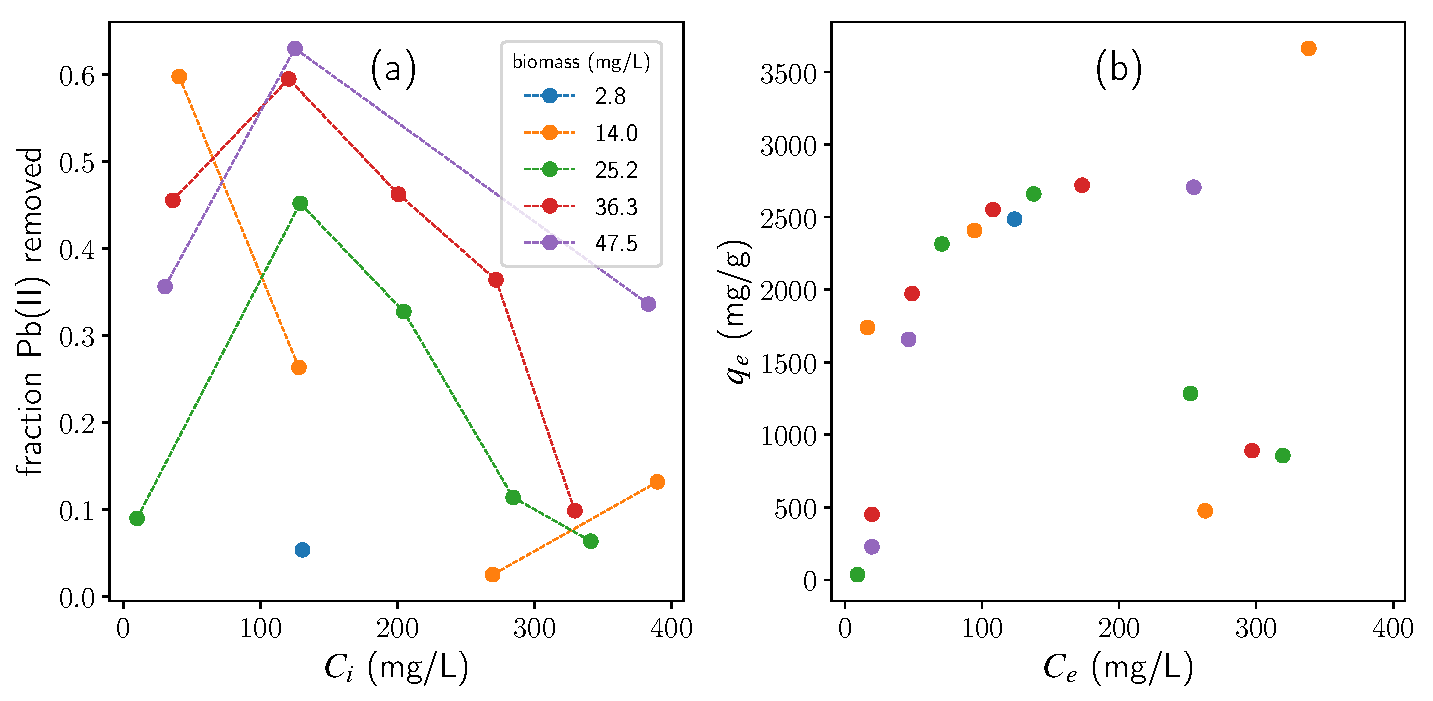
\includegraphics[width=1\linewidth]{Experimental/Pics/conc-vs-rem}
	\caption{The effects of biomass concentration and initial Pb(II) concentration on Pb(II) removal (a) and adsorption capacity (b). The legend shows dry biomass concentration and is shared between both plots.}
	\label{fig:conc-vs-rem}
\end{figure}






\section{Titration}

\subsection{Introduction}




\subsection{Materials and methods}

Acid-base titrations of prepared cultures were performed using an autotitrator (Metrohm 848 Titrino Plus). 

Standard solutions of \SI{0.1}{M} \ce{HNO3} and  \SI{0.1}{M} NaOH were used.

Cells prepared 
dynamic equivalence point titration with autotitrator (Metrohm 848 Titrino Plus).   stability of 50.0 mV/min

100 mL samples purged for 5 min with N2 and maintained throughout experiment.
temp control at 37 +- 1 Celsius
0.1 M NaOH and HNO3
acid added until a pH of 4 reached, increased with NaOH until 10. pH range outside causes cell damage (less than 3) and lysis (greater than 10) \parencite(Kapetas2011).

\subsection{Results and discussion}

\section{Adsorption kinetics}
\section{Adsorption equilibrium}

	
	\printbibliography[title=References, heading=bibintoc]
	
\end{document}